\documentclass[12pt]{article}
\usepackage[top=3cm, left=3cm, right=3cm, bottom=3cm]{geometry}
\usepackage{floatrow}
\usepackage[utf8]{inputenc}
\usepackage[english]{babel}
\usepackage{graphicx}
\usepackage[T1]{fontenc}
\usepackage{amsmath, amssymb}
\usepackage{natbib}
\usepackage{float}
\floatstyle{plaintop}
\restylefloat{table}
\usepackage{multirow}
\usepackage{parskip}
\usepackage{times}
\usepackage[font=small,labelfont=bf]{caption}
\usepackage{subcaption}
\linespread{1.05}
\usepackage[bottom]{footmisc}
\usepackage{hyperref}
\usepackage{multicol}
\usepackage{lipsum}
\usepackage{authblk}
\usepackage{dcolumn}
\usepackage{animate}
\usepackage{multimedia}
\usepackage{media9}
\usepackage[Export]{adjustbox}
\usepackage{tabularx}
\usepackage{cellspace}
\usepackage{longtable}
\usepackage{booktabs}
\usepackage{xspace} % Added to ensure \elide compiles correctly
\usepackage{tikz}
\usepackage{bm}
\usetikzlibrary{positioning, decorations.pathreplacing, calc, arrows.meta,fit,backgrounds}
\usepackage{xcolor}
\definecolor{cgrey}{HTML}{D9D9D9}  
\definecolor{cgreen}{HTML}{33A02C}           
\definecolor{cblue}{HTML}{1F78B4}  

\setlength\cellspacetoplimit{6pt}
\setlength\cellspacebottomlimit{0pt}
\renewcommand\tabularxcolumn[1]{>{\centering\arraybackslash}S{p{#1}}}

\DeclareCaptionLabelSeparator{pipe}{ $\textbf{|}$ }% or \vert

\let\oldnl\nl
\newcommand{\nonl}{\renewcommand{\nl}{\let\nl\oldnl}}

\newcommand{\hrulealg}[0]{\vspace{1mm} \hrule \vspace{1mm}}

\usepackage[title]{appendix}
\usepackage{algorithm2e}

\DeclareMathOperator*{\argmin}{arg\,min}
\usepackage{caption}

\usepackage{marvosym}

\usepackage{algorithmic}

\makeatletter
\renewcommand{\@algocf@capt@plain}{above}% formerly {bottom}
\makeatother

\newcommand*\elide{\textup{[\,\dots]}\xspace}

\providecommand{\keywords}[1]
{
  \vspace{0.5cm}
  \small	
  \textbf{\textit{Keywords---}} #1
}

\newcommand{\minus}{\scalebox{0.75}[1.0]{$-$}}
\newcommand{\overbar}[1]{\mkern 1.5mu\overline{\mkern-1.5mu#1\mkern-1.5mu}\mkern 1.5mu}

\makeatletter
% Make the FIRST footnote symbol an envelope (instead of *)
\renewcommand{\@fnsymbol}[1]{%
  \ifcase#1\or\Letter\or\dagger\or\ddagger\or\mathsection\or\mathparagraph\or\|\or**\or\dagger\dagger\or\ddagger\ddagger\else\@arabic{#1}\fi
}
\makeatother

\makeatletter
\let\orig@makefntext\@makefntext
\newcommand{\restore@makefntext}{\let\@makefntext\orig@makefntext}

\newcommand{\titlefootmarkscale}{1.85} % adjust (e.g., 1.30–1.60)

\newcommand{\settitle@makefntext}{%
  \renewcommand{\@makefntext}[1]{%
    \parindent 1em\noindent
    \hb@xt@1.8em{\hss\textsuperscript{\scalebox{\titlefootmarkscale}{\@thefnmark}}}%
    ##1%
  }%
}
\makeatother
%%%%%%%%%%%%%%%%%%%%%%%%%%%%%%%%%%%%%%%%%

\title{\textbf{Anticipating Continued Global Fertility Decline via Neural Forecasting}}

\author[1,2]{Daniel Ciganda\thanks{\href{mailto:ciganda@demogr.mpg.de}{ciganda@demogr.mpg.de}}}
\author[2]{Facundo Morini}
\author[3]{Francisco Piriz}

\affil[1]{\small Max Planck Institute for Demographic Research}
\affil[2]{\small Statistics Institute, University of the Republic}
\affil[3]{\small Digital Sense}

\date{}

\begin{document}

\makeatletter
\settitle@makefntext
\makeatother
\maketitle
\makeatletter
\restore@makefntext
\makeatother

\begin{abstract}
\noindent The accelerating shift toward low and ultra-low fertility has intensified the debate over whether countries now undergoing rapid decline are approaching stabilization or entering a more persistent low-fertility regime. Existing projection systems answer that question differently because they embed different assumptions about recovery and about the role of external drivers. To provide an empirical benchmark in this debate, we introduce NeuralTFR, an endogenous global forecasting framework based on a recurrent neural network. Drawing on a harmonized panel of historical fertility series from 196 countries and territories, the model pools cross-country information to learn demographic momentum and generate distribution-free prediction intervals via multi-quantile regression. Evaluated on a held-out period (2009--2023), NeuralTFR outperforms a Naive Drift baseline and improves on the point-forecast accuracy of BayesTFR, the United Nations' Bayesian Hierarchical Model, while maintaining competitive uncertainty calibration. In forward projections to 2040, NeuralTFR points to broader exposure to low and very low fertility than BayesTFR, suggesting weaker support for near-term stabilization while still falling short of the most severe decline paths predicted by the Global Burden of Disease team.
\end{abstract}

\keywords{Total Fertility Rate, Global Neural Forecasting, Recurrent Neural Networks, Quantile Regression, Probabilistic Forecasting, Continued Fertility Decline}\footnote{An interactive visualizer for the projection comparisons is available at \url{https://dciganda.github.io/NeuralTFR_visualizer/}.}

\clearpage

% ==========================================
% 1. INTRODUCTION
% ==========================================
\section{Introduction}

The accelerating global transition toward low and ultra-low fertility poses profound challenges to economic growth, welfare systems, and geopolitical stability. Anticipating the depth and duration of this demographic shift depends upon robust projections of the Total Fertility Rate (TFR), a central challenge in demographic forecasting. A primary controversy in this context revolves around whether countries currently experiencing rapid declines will eventually stabilize and undergo a moderate recovery, or whether they are entering a more persistent low-fertility regime \citep[see, e.g.,][]{basten2014future}.

Global demographic forecasting is currently shaped by three major institutional approaches: the United Nations Population Division \citep{un2024wpp}, the Wittgenstein Centre for Demography and Global Human Capital \citep{kc2024updating}, and the Global Burden of Disease (GBD) team \citep{gbd2024global}. These paradigms differ markedly in both methodology and projected outcomes, reflecting different assumptions about post-transitional fertility, the role of expert judgment, and the importance of exogenous drivers. These disagreements are not simply methodological. They reflect a fundamental gap in demographic knowledge: the post-transitional fertility landscape has been observed in only a handful of countries over a limited period \citep{goujon2025}, so the assumptions that drive long-run projections operate with limited empirical guidance. This raises a natural question: what do recent fertility trajectories suggest when projections depend less on recovery assumptions, external covariates, and expert adjustment?

To address that question, we introduce NeuralTFR, a global forecasting framework for the Total Fertility Rate built around an encoder-decoder architecture with Gated Recurrent Units (GRUs). Our approach formulates demographic projection as an autoregressive sequence-to-sequence task for forecasting multiple steps ahead. Rather than fitting isolated time-series models for each country, it uses a cross-series learning strategy. By jointly training a single model on a harmonized panel of historical fertility series from 196 countries and territories, NeuralTFR extracts shared, non-linear dynamics of the fertility transition directly from observed trajectories. The decoder is trained via multi-quantile regression, allowing the framework to generate distribution-free prediction intervals without relying on restrictive parametric assumptions or the computational burden of traditional Bayesian models.

By isolating the endogenous momentum of historical fertility trends, this framework yields two primary contributions:

First, methodologically, we show that a fully endogenous deep learning approach can perform strongly in demographic forecasting. Here, endogenous means that the model conditions on past fertility trajectories, without relying on exogenous socioeconomic covariates or expert adjustment, and that multi-step forecasts are generated autoregressively from the model's own learned dynamics rather than from externally imposed recovery paths. Evaluated on a fully held-out period (2009--2023), NeuralTFR outperforms a Naive Drift benchmark and improves on the point-forecast accuracy of the UN's BayesTFR model, while maintaining competitive empirical interval coverage.

Second, substantively, we provide a purely data-driven assessment of global fertility trajectories out to 2040. Our results suggest broader exposure to low and very low fertility than the United Nations projects, while still falling short of the most severe decline paths projected by the GBD framework. In that sense, when the global set of fertility trajectories is allowed to speak for itself, it offers limited support for either a near-term soft landing or the most severe decline scenarios currently published.

\section{Previous Work}

Global demographic forecasting is currently dominated by three major institutional approaches. These models diverge significantly in their results, reflecting different ways of specifying post-transitional fertility and its long-run evolution.

The first, and most widely adopted, is the probabilistic framework used by the United Nations Population Division \citep{un2024wpp}, which relies on the Bayesian Hierarchical Model (BayesTFR) developed by Raftery, \v{S}ev\v{c}ikova, Alkema and colleagues \citep{alkema2011probabilistic,raftery2014bayesian, raftery2023probabilistic}. This model partitions the fertility transition into distinct phases. Its post-transition phase (Phase III) models fertility as an autoregressive AR(1) process that reverts to a country-specific long-term asymptote. Because this asymptote is informed by a global prior derived from countries that have previously experienced fertility recoveries, the model builds in eventual stabilization and a mean-reverting rebound. For instance, the UN explicitly assumes that fertility in countries with already-peaked populations will gradually rebound to an average of 1.4 births per woman by 2100 \citep{un2024wpp}. Reflecting this expectation of recovering fertility, the UN anticipates the most conservative demographic decline, forecasting a global population of 10.2 billion by 2100.

The second approach, developed by the Wittgenstein Centre for Demography and Global Human Capital (IIASA/VID), uses multi-state cohort-component models that emphasize educational stratification \citep{lutz2014world, lutz2018demographic,kc2024updating}. To define long-term fertility asymptotes, this model relies on panels of demographic experts rather than automated time-series extrapolation. Drawing on concepts like the low-fertility trap, the IIASA model anticipates the persistence of low fertility and projects stabilization at levels generally lower than those assumed by the UN. Their most recent assessment (WIC2023) remains close to the United Nations over much of the overlapping horizon while projecting a global population of 9.9 billion by 2100 \citep{kc2024updating}. However, this approach depends heavily on subjective expert elicitation to set long-term bounds.

A third approach was developed by the Global Burden of Disease (GBD) team at the Institute for Health Metrics and Evaluation (IHME). The GBD model projects fertility using an ensemble approach with four covariates: female educational attainment, contraceptive met need, under-5 mortality, and population density in habitable areas \citep{gbd2024global}. Assuming these socio-economic and environmental drivers will continue to suppress birth rates, the GBD model projects a steeper and more sustained demographic decline than the UN. In their 2020 models, this resulted in a global population forecast of 8.8 billion by 2100, which is 1.4 billion people fewer than the UN estimate \citep{ihme2020, un2024wpp}. However, this method has faced heavy criticism within the demographic community. Initial concerns raised by over 170 population scientists in \textit{The Lancet} \citep{gietel2020letter} were further detailed by \cite{gietel2020uncertain}, who demonstrated that the GBD framework relies on inaccurate baseline data, imposes arbitrary fertility bounds, and lacks a suitable analytical framework for post-transitional, low-fertility societies.

A central challenge in fertility forecasting is that individual country series are often short and heterogeneous, while the broader panel contains shared temporal structure that can inform multi-step prediction. This is precisely the kind of forecasting problem in which recurrent neural networks have proven useful in other applied settings, by pooling information across related series while capturing non-linear temporal dynamics. Successful applications span inflation forecasting \citep{paranhos2025inflation}, e-commerce sales-demand forecasting \citep{bandara2019sales}, and financial market prediction \citep{fischer2018lstm}. The forecasting literature has also produced influential recurrent architectures such as DeepAR for probabilistic forecasting \citep{salinas2020deepar}, Smyl's hybrid ES-RNN model \citep{smyl2020hybrid}, and LSTNet for multivariate forecasting tasks \citep{lai2018modeling}. In demography, however, deep learning has been adopted more cautiously. The most successful applications of deep neural networks to demographic data have emerged within actuarial science, specifically in mortality forecasting. For instance, \citet{nigri2019deep} integrated Long Short-Term Memory (LSTM) networks into the classic Lee-Carter framework to forecast the mortality time index, demonstrating that recurrent architectures capture non-linear trends much more effectively than standard ARIMA processes. Similarly, \citet{beyaztas2022machine} employed machine learning-based forecasting strategies to predict principal component scores within a functional time series approach to age-specific mortality. More recently, the field has seen a broader adoption of fully deep architectures, such as Convolutional Neural Networks and Transformers, that directly model the age-period-cohort surface and leverage cross-population data \citep{zheng2025brief}. These multi-population deep learning models consistently outperform traditional stochastic baselines by learning shared demographic dynamics across populations \citep{park2025next}. 

These developments suggest that fertility forecasting may also benefit from recurrent global architectures, especially when the goal is to learn common dynamics across countries rather than fit isolated models to each series. The neural forecasting framework proposed in this paper directly addresses this gap. By modeling the complex dynamics of global fertility exclusively from historical time series, it provides a complementary empirical reference point alongside existing projection frameworks.

% ==========================================
% 3. DATA AND EMPIRICAL STRATEGY
% ==========================================
\section{Data and Empirical Strategy}

As discussed in the previous section, the appeal of recurrent global models in this setting lies in their ability to pool information across related series. That feature is especially important in macro-demographic forecasting, where annual observations remain scarce for any single country. Complex models, particularly neural networks, risk severe overfitting when trained on short, partitioned time series in isolation. To address this, we constructed a pooled, harmonized global dataset. By utilizing a Global Forecasting Model (GFM) approach \citep{januschowski2020criteria, montero2021principles}, the neural network simultaneously learns the shared, underlying dynamics of the demographic transition across multiple distinct trajectories.

\subsection{Data Sources and Harmonization}

The dataset is built from historical TFR estimates published by the United Nations Population Division \citep{un2024wpp}. We begin from 201 candidate countries and territories. From this pool, we retain all series with empirical annual TFR observations. Five entities, Sudan, Western Sahara, Sri Lanka, State of Palestine, and North Macedonia, appear only as modeled historical values rather than empirical observations, and are therefore not used for model fitting. The resulting dataset contains 196 countries and territories and covers the full empirical UN sample.

We use all available empirical country-year observations and, when multiple reports based on different data sources or estimation procedures exist for the same country-year, we take their median. Interior gaps are filled by linear interpolation, accounting for 465 country-year values, or 3.4\% of the final dataset. A limited smoothing rule is applied to series flagged as outliers on gap frequency, cross-source disagreement, or year-to-year volatility. Appendix~\ref{app:smoothing_ablation} describes the rule in detail and reports robustness checks in which this step is removed.

\subsection{Preprocessing and Global Standardization}

Prior to model input, we apply two transformations to the raw TFR series to stabilize the learning process and facilitate convergence. First, a natural logarithmic transformation is applied to the raw TFR values to compress the data range. 

Second, we implement a global standardization strategy. Rather than normalizing each time series individually, a standard scaler is fitted on the entire training set to compute a global mean ($\mu_{\text{global}}$) and standard deviation ($\sigma_{\text{global}}$). The standardized value $z_{i,t}$ is then calculated as:
\begin{equation}
    z_{i,t} = \frac{y_{i,t}^{\prime} - \mu_{\text{global}}}{\sigma_{\text{global}}}
\end{equation}
where $y_{i,t}^{\prime}$ represents the log-transformed TFR for geographic entity $i$ at time step $t$.

This global approach preserves the relative magnitude differences between countries. Unlike individual scaling, which would force all series to a common scale and potentially obscure the distinction between high and low fertility regimes, global scaling maintains the structural hierarchy of the data. This allows the model to distinguish between high- and low-fertility regimes while maintaining the numerical stability of standardized inputs.

\subsection{Temporal Structuring via Sliding Windows}

Once transformed, the time series are converted into input-output pairs suitable for supervised learning using a sliding window approach. For a given geographic entity $i$ and a specific time step $t$, the data is partitioned into two sequences:
\begin{itemize}
    \item \textbf{Encoder Sequence (Input):} A historical context window of length $L_{\text{enc}}$ defined as $X_{i,t} = \{z_{i,t-L_{\text{enc}}+1}, \dots, z_{i,t}\}$.
    \item \textbf{Decoder Sequence (Target):} A future horizon of length $L_{\text{pred}}$ (15 years) defined as $Y_{i,t} = \{z_{i,t+1}, \dots, z_{i,t+L_{\text{pred}}}\}$.
\end{itemize}

The window shifts sequentially by one time step ($s=1$) through the time series of each country. This sliding-window strategy generates thousands of training instances, capturing diverse temporal dynamics from both the onset and the stabilization phases of the fertility transition.

In the implemented specification, each encoder step combines the current standardized TFR with lagged fertility values at 2, 4, and 6 years, while a learned country embedding is supplied as a static categorical input.

To increase the model's exposure to very low-fertility dynamics during training, we apply a limited data-augmentation step to trajectories that reach an annual TFR of 1.3 or lower in the training data. For each selected trajectory, the 10 most recent training windows are duplicated once and perturbed with small Gaussian noise before being added to the training set. In the full-sample forecasting fit, this increases the number of training windows by about 8.5\%. This augmentation is used only during model fitting.

\begin{figure}[h!]
	\centering
	\begin{adjustbox}{max width=\linewidth}
	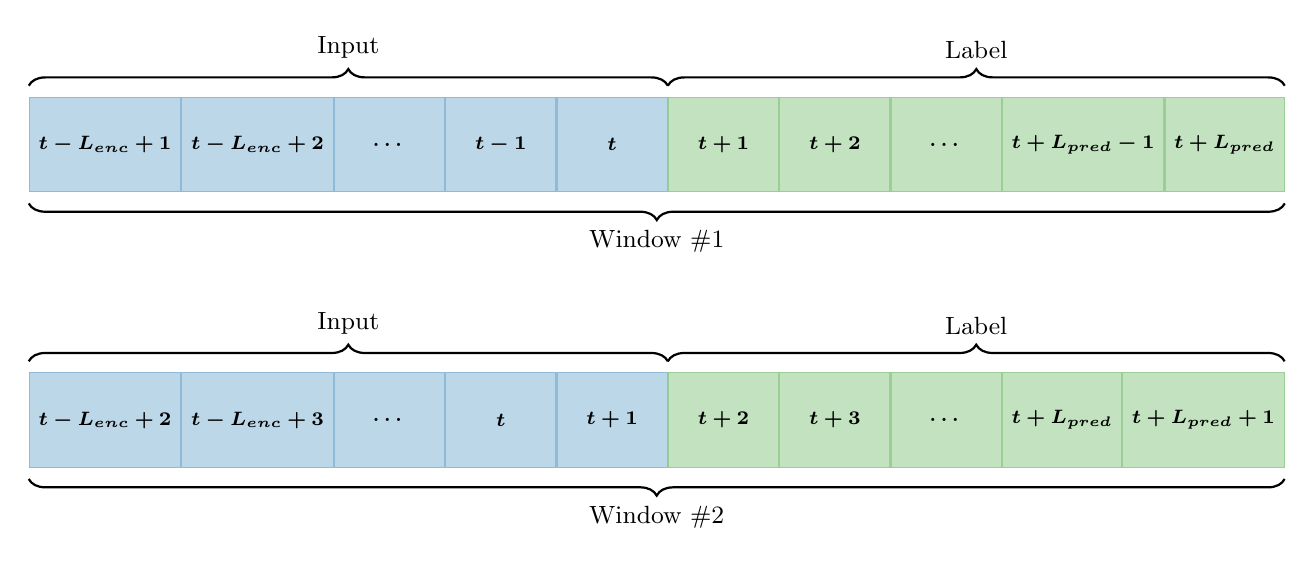
\begin{tikzpicture}[
	% Estilo para las cajas de tiempo
	inputbox/.style={
		draw,
		rectangle,
		draw=cblue!50,
		fill=cblue!30,
		minimum width=1.4cm,
		minimum height=1.2cm,
		align=center,
		font=\scriptsize\bfseries
	},
	labelbox/.style={
		draw,
		rectangle,
		draw=cgreen!50,
		fill=cgreen!30,
		minimum width=1.4cm,
		minimum height=1.2cm,
		align=center,
		font=\scriptsize\bfseries
	},
	% Estilo para las llaves decorativas
	brace/.style={
		decorate,
		decoration={brace, amplitude=6pt, raise=4pt},
		line width=0.8pt
	},
	% Estilo para el texto sobre las llaves
	bracelabel/.style={
		font=\small,
		above=10pt
	}
	]
	
	% --- Ventana de Datos #1 ---
	\begin{scope}[local bounding box=window1]
		% Nodos de la izquierda (Input)
		\node[inputbox] (t0) {$\bm{t-L_{enc}+1}$};
		\node[inputbox, right=0 of t0] (t1) {$\bm{t-L_{enc}+2}$};
		\node[inputbox, right=0 of t1] (dots1a) {\dots};
		\node[inputbox, right=0 of dots1a] (t22) {$\bm{t-1}$};
		\node[inputbox, right=0 of t22] (t23) {$\bm{t}$};
		
		% Nodos de la derecha (Label)
		\node[labelbox, right=0 of t23] (t24) {$\bm{t+1}$};
		\node[labelbox, right=0 of t24] (t25) {$\bm{t+2}$};
		\node[labelbox, right=0 of t25] (dots1b) {\dots};
		\node[labelbox, right=0 of dots1b] (t46) {$\bm{t+L_{pred}-1}$};
		\node[labelbox, right=0 of t46] (t47) {$\bm{t+L_{pred}}$};
		
		% Llaves superiores (Input y Label)
		\draw[brace] (t0.north west) -- (t23.north east) 
		node[midway, bracelabel] {Input};
		\draw[brace] (t24.north west) -- (t47.north east) 
		node[midway, bracelabel] {Label};
		
		% Llave inferior (Data window)
		\draw[brace] (t47.south east) -- (t0.south west) 
		node[midway, below=10pt, font=\small] {Window \#1};
	\end{scope}
	
	
	% --- Ventana de Datos #2 ---
	\begin{scope}[yshift=-3.5cm, local bounding box=window2]
		% Nodos de la izquierda (Input)
		\node[inputbox] (t0) {$\bm{t-L_{enc}+2}$};
		\node[inputbox, right=0 of t0] (t1) {$\bm{t-L_{enc}+3}$};
		\node[inputbox, right=0 of t1] (dots1a) {\dots};
		\node[inputbox, right=0 of dots1a] (t22) {$\bm{t}$};
		\node[inputbox, right=0 of t22] (t23) {$\bm{t+1}$};
		
		% Nodos de la derecha (Label)
		\node[labelbox, right=0 of t23] (t24) {$\bm{t+2}$};
		\node[labelbox, right=0 of t24] (t25) {$\bm{t+3}$};
		\node[labelbox, right=0 of t25] (dots1b) {\dots};
		\node[labelbox, right=0 of dots1b] (t46) {$\bm{t+L_{pred}}$};
		\node[labelbox, right=0 of t46] (t47) {$\bm{t+L_{pred}+1}$};
		
		% Llaves superiores (Input y Label)
		\draw[brace] (t0.north west) -- (t23.north east) 
		node[midway, bracelabel] {Input};
		\draw[brace] (t24.north west) -- (t47.north east) 
		node[midway, bracelabel] {Label};
		
		% Llave inferior (Data window)
		\draw[brace] (t47.south east) -- (t0.south west) 
		node[midway, below=10pt, font=\small] {Window \#2};
	\end{scope}
	
\end{tikzpicture}
	\end{adjustbox}
	\caption[Sliding Window Approach]{\textbf{Schematic representation of the Sliding Window approach.} The diagram illustrates how a continuous time series is sliced into input-output pairs. At each step $t$, a historical window of length $L_{enc}$ (Encoder, shown in blue) is used to predict a future horizon of length $L_{pred}$ (Decoder, shown in green). The window then shifts by one time step ($s=1$) to generate the subsequent training sample, ensuring the model learns from all available temporal transitions.}
	\label{fig:win_sld}
\end{figure}


% ==========================================
% 4. MODEL ARCHITECTURE
% ==========================================
\section{Model Architecture}

The core of our forecasting framework is a recurrent neural network (RNN) that maps an input sequence of historical observations to an output sequence of future projections. The architecture relies on two main components: the Gated Recurrent Unit (GRU) and an autoregressive encoder-decoder structure.

\subsection{Background: Gated Recurrent Units (GRU)}

Unlike traditional feed-forward networks that process inputs independently, RNNs maintain an internal hidden state that is updated sequentially, allowing the model to capture temporal dependencies. However, standard RNNs struggle to learn long-range dependencies due to the vanishing gradient problem \citep{hochreiter1997long}. 

To mitigate this, our architecture utilizes the Gated Recurrent Unit (GRU) introduced by \cite{cho2014learning}. The GRU is a streamlined variant of the Long Short-Term Memory (LSTM) cell that requires fewer trainable parameters while achieving comparable performance in sequence modelling tasks. 

The GRU controls the flow of information through two specific gating mechanisms: the update gate and the reset gate. For a given time step $t$, let $x_t$ denote the input vector and $h_{t-1}$ denote the hidden state from the previous time step. The operations within the GRU cell are formally defined by the following equations:

\begin{align}
    u_t &= \sigma(W_{xu} x_t + W_{hu} h_{t-1} + b_u) \label{eq:update_gate} \\
    r_t &= \sigma(W_{xr} x_t + W_{hr} h_{t-1} + b_r) \label{eq:reset_gate} \\
    \tilde{h}_t &= \tanh(W_{xh} x_t + W_{hh} (r_t \odot h_{t-1}) + b_h) \label{eq:candidate_state} \\
    h_t &= u_t \odot h_{t-1} + (1 - u_t) \odot \tilde{h}_t \label{eq:hidden_state}
\end{align}

Here, $u_t$ represents the update gate, which dictates how much of the previous hidden state $h_{t-1}$ is retained versus how much of the new candidate state $\tilde{h}_t$ is incorporated. The reset gate $r_t$ determines the extent to which past information is forgotten when computing the new candidate state. The matrices $W$ represent the trainable weight parameters, $b$ denotes the bias vectors, $\sigma$ is the logistic sigmoid activation function, and $\odot$ denotes the element-wise Hadamard product. By optimizing these gating parameters, the network autonomously learns to retain relevant long-term demographic momentum while discarding transient noise.

\subsection{The Sequence-to-Sequence Architecture}

To accommodate multi-step-ahead forecasting natively, we employ an encoder-decoder (Sequence-to-Sequence) architecture \citep{sutskever2014sequence}. This framework maps the historical conditioning range to the future prediction range without relying on independent models for each future time step.

\begin{enumerate}
    \item \textbf{The Encoder:} The encoder module processes the scaled historical input sequence step-by-step. Once the entire historical window of length $L_{\text{enc}}$ has been processed, the encoder outputs a final hidden state, denoted as $h_{\text{enc}}$. This context vector serves as a dense, compressed representation (embedding) of the country's entire historical fertility trajectory.
    \item \textbf{The Decoder:} The decoder module is initialized with the context vector $h_{\text{enc}}$ generated by the encoder. Its objective is to generate the forecast sequence over the prediction horizon $L_{\text{pred}}$. The decoder operates \textit{autoregressively}; it unrolls the future trajectory one step at a time, utilizing its own output from the previous step as the input for the subsequent step. 
\end{enumerate}

During the training phase, the autoregressive decoder utilizes a \textit{teacher forcing} mechanism. Rather than feeding the network's own potentially inaccurate predictions back into the model, the true observed values of the Total Fertility Rate are supplied as inputs to the subsequent steps. The probability of applying teacher forcing decays gradually as training progresses, ensuring the model stabilizes early while eventually learning to rely on its own generated sequence.


\subsection{Uncertainty Quantification via Quantile Regression and Ensembling}

A critical limitation of standard neural-network forecasting setups in macro-forecasting is that they are typically trained and used to produce deterministic point estimates. To support demographic planning and policy design, models must provide reliable prediction intervals. Our framework addresses this requirement through a dual approach: non-parametric quantile regression and ensembling.

The final layer of the decoder consists of a linear projection that maps the recurrent hidden states to a vector of size $Q$. Its entries correspond to a predefined set of target quantiles $\tau \in \{0.05,\allowbreak 0.10,\allowbreak 0.50,\allowbreak 0.90,\allowbreak 0.95\}$. Consequently, at each forecast step $h \in \{1, \dots, L_{\text{pred}}\}$, the model outputs a discrete approximation of the conditional distribution $P(y_{i,t+h} \mid X_{i,t})$. This design allows for the direct construction of 80\% and 90\% prediction intervals without imposing strict parametric assumptions, such as normality, on the error distribution. 

To optimize the network for probabilistic calibration, we train the model by minimizing the multi-quantile loss \citep{koenker1978regression}. For a single true observation $y_t$ and a predicted quantile value $\hat{y}_t^{(\tau)}$ targeting a specific probability $\tau \in (0,1)$, the loss function is defined as:
\begin{equation}
    \mathcal{L}_\tau(y_t, \hat{y}_t^{(\tau)}) = \max\Big(\tau(y_t - \hat{y}_t^{(\tau)}), (\tau - 1)(y_t - \hat{y}_t^{(\tau)})\Big)
\end{equation}

This mechanism relies on an asymmetric penalty scheme:
\begin{itemize}
    \item \textbf{High quantiles ($\tau > 0.50$):} Underestimating the true value incurs a heavier penalty than overestimating it. For example, when $\tau = 0.95$, underestimation is weighted by 0.95 and overestimation by 0.05. This asymmetry forces the model to push the prediction upward, establishing a reliable empirical upper bound.
    \item \textbf{Low quantiles ($\tau < 0.50$):} Overestimation is penalized more heavily than underestimation. For $\tau = 0.05$, this dynamic effectively pushes the prediction downward to act as a robust lower bound.
    \item \textbf{The median ($\tau = 0.50$):} The penalty is perfectly symmetric, rendering the optimization mathematically equivalent to minimizing the Mean Absolute Error (MAE).
\end{itemize}

The total objective function optimized during training is the sum of these asymmetric losses over all time steps in the prediction horizon $L_{\text{pred}}$ and across the complete set of target quantiles $Q$:
\begin{equation}
    \mathcal{L}_{\text{total}} = \sum_{k=1}^{L_{\text{pred}}} \sum_{\tau \in Q} \mathcal{L}_\tau(y_{t+k}, \hat{y}_{t+k}^{(\tau)})
\end{equation}

By jointly minimizing this objective across multiple quantiles, the neural network learns to construct a comprehensive and well-calibrated probabilistic envelope around the central demographic forecast. Throughout the paper, this central point forecast is defined as the median trajectory.

To stabilize the forecasts and account for the model's sensitivity to initial parameters, we implemented an ensemble strategy. The final probabilistic forecast for any given country is generated by taking the element-wise median of the quantile predictions from 10 structurally identical models, each trained independently utilizing a different random weight initialization seed and slightly varied hyperparameters to ensure model diversity.

\subsection{Optimization, Tuning, and Evaluation Strategy}

To prevent our highly parameterized neural network from overfitting the limited annual observations typical of national fertility series, we implemented a set of regularization strategies designed to isolate generalizable demographic momentum from historical noise. First, the global cross-learning strategy itself acts as a powerful structural regularizer. By training a single network on 196 diverse series simultaneously, the model is discouraged from overfitting to the idiosyncratic fluctuations of any individual country.

The network parameters were optimized using the Adaptive Moment Estimation (Adam) algorithm, augmented with a weight decay penalty (L2 regularization) to constrain parameter magnitudes. Furthermore, we implemented a dynamic step learning rate scheduler and an early stopping mechanism, halting training if the validation loss failed to improve over a predefined patience threshold.

Independent of regularization, the specific configuration of the network architecture critically impacts its learning efficiency and forecasting performance. To systematically identify the optimal configuration, hyperparameter tuning was conducted via Bayesian optimization using the \textit{Optuna} framework \citep{optuna_2019}. The search space evaluated the learning rate, the hidden state dimension of the GRU cells, the number of recurrent layers, and the training batch size.

To ensure a robust and unbiased evaluation of these configurations, and to ultimately assess the model's out-of-sample performance without look-ahead bias, we employed a strict temporal data partitioning and validation strategy. The global dataset was chronologically split into two distinct periods.

\noindent\textbf{Training and tuning partition ($t < 2009$):} Comprises all historical data up to the year 2008. This partition is used exclusively to learn the model parameters and tune hyperparameters. Within this partition, we utilized a rolling forecast origin cross-validation strategy. This temporal validation technique iteratively trains the model on an expanding historical window and evaluates it on the immediately subsequent period, strictly preventing data leakage while accurately simulating real-world forecasting conditions during the tuning phase.

\noindent\textbf{Test partition ($t \ge 2009$):} Comprises data from 2009 onwards. This partition is kept completely unseen during the training and tuning phases. It is used exclusively to evaluate the fully optimized model's generalization performance on future horizons.

% ==========================================
% 5. FORECAST EVALUATION
% ==========================================
\section{Forecast Evaluation}

The out-of-sample evaluation period from 2009 to 2023 represents a highly challenging forecasting environment, characterized by the unexpected acceleration of ultra-low fertility in developed economies and shifting transition speeds in developing nations. The full dataset contains 196 countries and territories, of which 192 enter the holdout comparison.\footnote{Eritrea and the Syrian Arab Republic have no observed values after 2008; Kosovo and Jersey could not be obtained from the BayesTFR output files.} To assess how well NeuralTFR generalizes across these diverse trajectories, we benchmark its predictive accuracy over these 192 entities for which comparable NeuralTFR, BayesTFR, and Naive Drift predictions are jointly available. The first reference model is Naive Drift, a simple but often effective univariate random-walk-with-drift specification that we use as a statistical baseline. It establishes a transparent minimum performance threshold and allows us to evaluate whether the computational complexity of a global neural network yields tangible improvements over straightforward local extrapolation. The second is the Bayesian Hierarchical Model (BayesTFR), an established demographic forecasting framework and the state-of-the-art standard utilized by the United Nations Population Division, which serves as our primary structural and probabilistic benchmark.

Given the differences in absolute fertility levels across our panel of 192 countries, standard scale-dependent metrics like Root Mean Squared Error (RMSE) can be skewed by errors in high-fertility regions. Therefore, alongside RMSE, we utilize scale-independent metrics, namely the Symmetric Mean Absolute Percentage Error (sMAPE) and the Root Mean Squared Scaled Error (RMSSE). Point forecast accuracy is evaluated using the median forecast for each model. Furthermore, to evaluate the probabilistic distributions generated by the models, we report the Continuous Ranked Probability Score (CRPS), empirical 90\% interval coverage, and the Mean Prediction Interval Width (MPIW) for the 90\% interval.

\subsection{Point Forecast Accuracy}

The evaluation of point forecast accuracy shows that the global deep learning approach outperforms both the Naive Drift baseline and the Bayesian hierarchical framework. As illustrated by the distribution of point metrics across the test set (Figure~\ref{fig:point_metrics}), NeuralTFR demonstrates robust generalization capabilities. 

For RMSE, sMAPE, and RMSSE, the median error for NeuralTFR is visibly lower than that of BayesTFR. Beyond the central tendency, the most striking feature of the neural network's performance is the reduced variance and the mitigation of extreme errors. The interquartile ranges are narrower and the upper whiskers are significantly compressed compared to the probabilistic baseline. This indicates that NeuralTFR does not merely improve the average forecast but substantially reduces the risk of extreme prediction failures that can occur in traditional models. 

\begin{figure}[H]
\centering
\setlength{\tabcolsep}{0pt}
\renewcommand{\arraystretch}{1.0}
\begin{tabular}{@{}m{0.085\textwidth}@{\hspace{0.008\textwidth}}m{0.905\textwidth}@{}}
    \centering{\small (a) RMSE} &
    
\includegraphics[width=\linewidth,height=0.205\textheight,keepaspectratio]{../../../compute/results/evaluation/metrics/metrics_rmse.pdf} \\
    \centering{\small (b) sMAPE} &
    
\includegraphics[width=\linewidth,height=0.205\textheight,keepaspectratio]{../../../compute/results/evaluation/metrics/metrics_smape.pdf} \\
    \centering{\small (c) RMSSE} &
    
\includegraphics[width=\linewidth,height=0.205\textheight,keepaspectratio]{../../../compute/results/evaluation/metrics/metrics_rmsse.pdf}
\end{tabular}
\caption{\textbf{Distribution of point forecast evaluation metrics across the 192 test countries for the 2009--2023 out-of-sample period.} Lower values indicate superior predictive accuracy. NeuralTFR consistently exhibits lower median error and reduced dispersion relative to the benchmark models. When reported in the panel legend, the Wilcoxon $p$-value refers to a paired signed-rank test on country-level errors comparing the model with the lowest median error to the second-best model for that metric.}
\label{fig:point_metrics}
\end{figure}

\subsection{Probabilistic Calibration and Sharpness}

In macro-demographic planning, point estimates are insufficient without a reliable quantification of uncertainty. While BayesTFR generates probabilistic forecasts via Markov Chain Monte Carlo (MCMC) simulations, our architecture approximates the predictive distribution empirically through the non-parametric multi-quantile loss.

Panel (a) of Figure~\ref{fig:uncertainty_metrics} shows the Continuous Ranked Probability Score (CRPS), which compares the full predictive distribution with the realized outcome and is minimized in expectation when the forecast distribution coincides with the true one. Lower values therefore indicate better overall probabilistic accuracy, combining calibration, understood here as agreement between nominal and empirical frequencies, with sharpness, understood as concentration of the predictive distribution. In this panel, NeuralTFR attains a noticeably lower median CRPS and a tighter distribution than BayesTFR. Panel (b) reports, for each country, the empirical share of held-out observations that fall within the nominal 90\% prediction interval, so values near 90\% indicate well-calibrated uncertainty. NeuralTFR's distribution is shifted upward and more often lies near or above the nominal target, indicating that its intervals more reliably contain the realized path, although values above 90\% suggest that the intervals may be somewhat wider than required for nominal calibration in part of the sample. BayesTFR more often falls below the nominal level, while still attaining nominal coverage for many countries.

\begin{figure}[H]
\centering
\setlength{\tabcolsep}{0pt}
\renewcommand{\arraystretch}{1.0}
\begin{tabular}{@{}m{0.085\textwidth}@{\hspace{0.008\textwidth}}m{0.905\textwidth}@{}}
    \centering{\small (a) CRPS} &
    
\includegraphics[width=\linewidth,height=0.205\textheight,keepaspectratio]{../../../compute/results/evaluation/metrics/metrics_crps.pdf} \\
    \centering{\small (b) Cov.\ 90\%} &
    
\includegraphics[width=\linewidth,height=0.205\textheight,keepaspectratio]{../../../compute/results/evaluation/metrics/metrics_coverage_90.pdf} \\
    \centering{\small (c) MPIW 90\%} &
    
\includegraphics[width=\linewidth,height=0.205\textheight,keepaspectratio]{../../../compute/results/evaluation/metrics/metrics_mpiw_90.pdf}
\end{tabular}
\caption{\textbf{Distribution of probabilistic calibration and sharpness metrics across the 192 test countries.} Each point corresponds to a country-level summary metric computed over the held-out years. CRPS jointly summarizes calibration and sharpness, the coverage panel compares empirical 90\% interval coverage to the nominal target, and MPIW 90\% reports the width of the corresponding prediction interval. The Wilcoxon $p$-value summarizes the paired comparison between the two models with the most favorable median values for that metric.}
\label{fig:uncertainty_metrics}
\end{figure}

Panel (c) reports the Mean Prediction Interval Width (MPIW) for the 90\% interval, which provides a direct view of sharpness because narrower intervals are desirable only if coverage remains adequate. BayesTFR shows a narrower median interval width, but also a more pronounced upper tail, indicating that it often produces sharper central intervals while occasionally expanding uncertainty substantially for particular populations. NeuralTFR instead yields more stable interval widths across countries, with less dispersion but somewhat wider typical intervals. Combined with the coverage results, this suggests a trade-off between median sharpness and stability in uncertainty quantification. Taken together, CRPS, coverage, and MPIW indicate that the non-parametric multi-quantile loss yields probabilistic forecasts that are well calibrated and maintain a useful balance between coverage and sharpness across countries.

\subsection{Comparative Performance Across TFR Trajectories}

To complement the cross-country metric comparisons in Figures~\ref{fig:point_metrics} and \ref{fig:uncertainty_metrics}, we inspect representative out-of-sample series from the same evaluation exercise in order to assess the model's strengths and limitations in handling specific TFR scenarios. The selected countries are illustrative rather than exhaustive, but they represent recurring trajectory patterns that help clarify where the model performs well and where it struggles.

Figure~\ref{fig:scenario_strengths} highlights cases in which NeuralTFR benefits from its flexible, data-driven structure. In Italy and Greece, fertility remains entrenched at very low levels and fails to display the recovery implied by BayesTFR's structural dynamics; as a result, BayesTFR drifts upward too quickly, while NeuralTFR remains much closer to the realized path. Canada and Belgium show a related pattern in which fertility decline resumes after a temporary plateau. Here again the neural model adapts more readily to renewed downward momentum, whereas BayesTFR remains systematically too high. Similar patterns also appear in Australia, Denmark, and New Zealand, suggesting that NeuralTFR is particularly strong when post-transition decline persists rather than reverting.

\begin{figure}[H]
\centering

\includegraphics[width=0.97\linewidth]{../../../compute/results/plots/fig5_scenarios_strengths.pdf}
\caption{\textbf{Representative held-out trajectories where NeuralTFR better captures persistent or renewed fertility decline, 2009--2023.} The shaded background marks the out-of-sample evaluation window. Observed history before 2009 is shown in lighter grey, held-out observations in darker grey, and the colored ribbons denote the 90\% prediction intervals around the median forecasts from NeuralTFR and the re-estimated BayesTFR benchmark. Italy and Greece illustrate persistent very low fertility without recovery, while Canada and Belgium show renewed decline after a temporary plateau.}
\label{fig:scenario_strengths}
\end{figure}

Figure~\ref{fig:nordics_us} extends this comparison to the United States and selected Nordic countries, where fertility declined markedly after a period of relative stability during the evaluation window.

\begin{figure}[H]
\centering

\includegraphics[width=0.97\linewidth]{../../../compute/results/plots/fig4_nordics_us_subset.pdf}
\caption{\textbf{Held-out trajectories for the United States and selected Nordic countries, 2009--2023.} These countries experienced an unanticipated fertility decline during the evaluation window. The shaded background marks the out-of-sample period. Observed history before 2009 is shown in lighter grey, held-out observations in darker grey, and the colored ribbons denote the 90\% prediction intervals around the median forecasts from NeuralTFR and BayesTFR.}
\label{fig:nordics_us}
\end{figure}

Figure~\ref{fig:scenario_limitations} shows the main settings in which the purely data-driven model becomes less reliable. South Korea represents an out-of-distribution collapse: fertility falls to levels well below the range seen in most of the training panel, and although NeuralTFR still tracks the decline better than BayesTFR, it fails to anticipate the full depth of the collapse. Kazakhstan and Uzbekistan illustrate a different limitation, namely strong rebounds after earlier decline. In these cases the neural model continues extrapolating downward momentum, while BayesTFR is closer to the realized reversal. Romania shows a similar problem in lower-fertility Europe: when fertility turns upward, NeuralTFR continues to project decline and misses the rebound. These examples clarify that the model's main weakness is not ordinary forecast noise, but difficulty with genuinely novel breaks from the historical patterns it has learned.

\begin{figure}[H]
\centering

\includegraphics[width=0.97\linewidth]{../../../compute/results/plots/fig5_scenarios_limitations.pdf}
\caption{\textbf{Representative held-out trajectories where NeuralTFR struggles under unprecedented collapse or rebound, 2009--2023.} The shaded background marks the out-of-sample evaluation window. Observed history before 2009 is shown in lighter grey, held-out observations in darker grey, and the colored ribbons denote the 90\% prediction intervals around the median forecasts from NeuralTFR and the re-estimated BayesTFR benchmark. South Korea illustrates an unprecedented ultra-low collapse, while Kazakhstan, Uzbekistan, and Romania show rebounds or reversals that the data-driven model does not anticipate well.}
\label{fig:scenario_limitations}
\end{figure}

% ==========================================
% 5. GLOBAL PROJECTIONS TO 2040
% ==========================================
\section{Comparative Global Projections}

Having validated NeuralTFR against BayesTFR on the held-out period, we next turn to the published forward projections currently informing the global demographic debate. For this exercise, we compare NeuralTFR against the published BayesTFR-based United Nations projections and against the Global Burden of Disease (GBD) projections. Although the Wittgenstein Centre projections (WIC2023) provide an important benchmark, we do not include them in the main comparison because their published forecasts remain close to those of the United Nations over the overlapping horizon and are available only in five-year intervals. To keep the comparison consistent across institutions, the main text focuses on the 151 countries for which published projections are available from all three models.

At the aggregate level, all three approaches project continued fertility decline, but they imply markedly different futures. Over most of the projection horizon, the BayesTFR path is the most conservative and implies the shallowest decline. At the opposite extreme, the GBD projections imply the most severe and persistent decline. NeuralTFR lies between these two benchmarks, pointing to deeper and more widespread low fertility than in the United Nations trajectory without reproducing the full severity of the GBD scenario.

\begin{figure}[H]
\centering
\begin{subfigure}[t]{0.44\linewidth}
\centering

\includegraphics[width=\linewidth]{../../../compute/results/plots/forecast_weighted_trajectory_5year.pdf}
\caption{Population-weighted average TFR by five-year interval.}
\end{subfigure}
\hfill
\begin{subfigure}[t]{0.54\linewidth}
\centering

\includegraphics[width=\linewidth]{../../../compute/results/plots/forecast_exclusive_category_bars_last_available.pdf}
\caption{Share of countries by TFR category at the last available projected year.}
\end{subfigure}
\caption{\textbf{Aggregate projection comparison for the 151-country comparison sample, 2025--2040.} Panel (a) reports the population-weighted average TFR within each five-year interval. Panel (b) summarizes the proportion of countries in mutually exclusive fertility categories at the last available projected year for each country.}
\label{fig:global_projection_comparison}
\end{figure}


Panel (b) shows that the main differences across models emerge below replacement level. NeuralTFR places a larger share of countries in the 1.3 to 1.5 range than either BayesTFR or GBD, while GBD allocates the largest share to the most extreme category below 1.3. BayesTFR, in contrast, leaves the largest share of countries at or above replacement level.

These aggregate distributions still conceal substantial regional heterogeneity. Figures~\ref{fig:regional_thresholds_1} and \ref{fig:regional_thresholds_2} therefore disaggregate the country-level projections at the last available projected year for each country across coherent regional groupings. The shaded bands mark replacement fertility ($\mathrm{TFR} < 2.1$), very low fertility ($\mathrm{TFR} < 1.5$), and ultra-low fertility ($\mathrm{TFR} < 1.3$), while the country-level markers show how the three projection models position individual series within those ranges.

Figure~\ref{fig:regional_thresholds_1} shows that the broad aggregate ordering is reproduced across Europe and Asia, but with important regional differences. In Northern and Western Europe, the three projections often remain relatively close together and mostly cluster between 1.3 and 1.8, implying continued low fertility but limited disagreement about the depth of the decline. By contrast, Southern and Eastern Europe displays a wider gap between the BayesTFR path and the lower NeuralTFR and GBD trajectories. That contrast is especially visible in countries such as Portugal, Romania, Bulgaria, and Slovakia, where NeuralTFR falls well below BayesTFR, while GBD is lowest in cases such as Bosnia-Herzegovina, Poland, and Italy. East and Southeast Asia remains entrenched in very low fertility under all three models, with South Korea, Singapore, China, Japan, and Thailand clustering close to or below the 1.3--1.5 bands. South and Central Asia shows a clearer separation, with BayesTFR typically highest for countries such as India, Nepal, Iran, and Uzbekistan, NeuralTFR in the middle, and GBD lowest.

\begin{figure}[H]
\centering

\includegraphics[width=\linewidth]{../../../compute/results/plots/forecast_threshold_ladder_regions_1_last_available.pdf}
\caption{\textbf{Regional fertility thresholds in Europe and Asia at the projection endpoint.} Each row corresponds to one country and each marker to one projection model, using each country's projection endpoint in the comparison sample. The shaded bands indicate replacement fertility ($\mathrm{TFR} < 2.1$), very low fertility ($\mathrm{TFR} < 1.5$), and ultra-low fertility ($\mathrm{TFR} < 1.3$). Southern and Eastern Europe displays the clearest departure of NeuralTFR from the BayesTFR path, while East and Southeast Asia remains concentrated in already very low fertility regimes across all three models.}
\label{fig:regional_thresholds_1}
\end{figure}

Figure~\ref{fig:regional_thresholds_2} shows broadly similar contrasts outside Europe and Asia, again with meaningful regional variation. In the Middle East and North Africa, BayesTFR generally remains closest to the upper part of the low-fertility range, whereas NeuralTFR and especially GBD place several countries lower at the projection endpoint. In the Americas, NeuralTFR frequently lies below BayesTFR while remaining above the GBD path, a pattern that is easy to see for countries such as Brazil, Ecuador, Peru, the Dominican Republic, Belize, and Panama. Oceania and Sub-Saharan Africa remain the most heterogeneous panels. Taiwan already occupies an ultra-low-fertility position, while countries such as Vanuatu, Ghana, Rwanda, and Tanzania remain above replacement fertility under all three models. Even in these more heterogeneous regions, the ordering is often informative, with NeuralTFR typically below BayesTFR and GBD lowest in many cases.

\begin{figure}[H]
\centering

\includegraphics[width=\linewidth]{../../../compute/results/plots/forecast_threshold_ladder_regions_2_last_available.pdf}
\caption{\textbf{Regional fertility thresholds in the Middle East, Oceania, the Americas, and Africa at the projection endpoint.} Each row corresponds to one country and each marker to one projection model, using each country's projection endpoint in the comparison sample. The shaded bands again denote replacement fertility ($\mathrm{TFR} < 2.1$), very low fertility ($\mathrm{TFR} < 1.5$), and ultra-low fertility ($\mathrm{TFR} < 1.3$). The Americas are mostly concentrated between 1.3 and 2.0, while Oceania and Africa show greater dispersion, including several countries that remain above replacement fertility under all three models.}
\label{fig:regional_thresholds_2}
\end{figure}


% ==========================================
% 6. CONCLUSION
% ==========================================
\section{Conclusion and Future Directions}

The broader question motivating this paper is the one at the center of current demographic debate: whether countries now experiencing rapid fertility decline are moving toward a moderate stabilization, or instead entering a more persistent low-fertility regime. Existing projection systems answer that question differently because they embed different assumptions about recovery, expert judgment, or exogenous socioeconomic drivers. NeuralTFR was developed as a deliberately empirical benchmark in that debate: an endogenous global model that learns from cross-country fertility histories without imposing demographic phases or long-run asymptotes, while still producing both point and probabilistic forecasts within a unified sequence-to-sequence framework.

Methodologically, the results show that a global deep learning approach can perform strongly in macro-demographic forecasting when evaluated on a fully held-out period. Across the 2009--2023 out-of-sample period, NeuralTFR outperforms both the Naive Drift baseline and BayesTFR on point forecast accuracy. It also yields probabilistic forecasts that are well calibrated and maintain a useful balance between coverage and sharpness through the non-parametric multi-quantile loss. The trajectory-based examples further show that these gains are especially visible when fertility decline persists or resumes after a temporary pause, while also clarifying the model's limits under abrupt reversals and other unusually difficult cases. Relative to the MCMC-based BayesTFR framework, NeuralTFR is also substantially cheaper to train and update computationally, making repeated re-estimation and scenario comparison more tractable.

Substantively, the 151-country forward comparison suggests that the central disagreement across projection systems is not whether fertility continues to decline, but how far and how fast that decline extends into very low-fertility regimes. BayesTFR remains the least aggressive benchmark over most of the projection horizon, while GBD implies the steepest deterioration. NeuralTFR points to broader exposure to low and very low fertility than BayesTFR overall, but it does not reproduce the full severity of the GBD scenario. Taken together, the comparison indicates that the momentum in recent fertility trajectories is difficult to reconcile with the relatively benign stabilization embedded in BayesTFR, while still falling short of supporting the much steeper deterioration implied by GBD.

\subsection*{Limitations and Future Directions}

The main limitation of a purely endogenous model is that it can only learn from the range of trajectories present in the historical record. As shown in the evaluation, NeuralTFR successfully captures renewed decline and persistent low fertility across a range of post-transition countries. It remained too cautious, however, in the face of South Korea's continued collapse toward ultra-low fertility and struggled more with abrupt reversals in parts of Central Asia, illustrating the difficulty of extrapolating genuinely unusual demographic behavior from past momentum alone.

A related limitation concerns forecast horizon. Because national annual fertility series are relatively short, extending the prediction horizon substantially would reduce the number of usable sliding windows and leave too little temporal variation for stable training. The current framework is therefore better suited to relatively short- and medium-run horizons than to very long-term projections, which remains an important direction for future work.

The present framework can be extended in two directions. One is architectural, by testing more flexible sequence models for long-range demographic dependencies. The other is substantive, by combining the endogenous neural baseline with selected exogenous covariates for conditional scenario analysis. More broadly, NeuralTFR should be understood not as a replacement for structural demographic models, but as a transparent empirical benchmark for assessing how strongly long-run fertility projections depend on the assumptions built into those models.

\subsection*{Reproducibility Statement}

The code, processed data, model outputs, and supporting resources needed to reproduce the empirical results are available at \url{https://github.com/dciganda/NeuralTFR}.

\appendix

\section{Smoothing Rule and Robustness Analysis}
\label{app:smoothing_ablation}

This analysis applies a limited smoothing step after annual country-year medians have been constructed and interior gaps have been filled by linear interpolation. This step is designed to stabilize trajectories that appear especially noisy while leaving the rest of the empirical panel unchanged. The smoothing decision is based on three diagnostics computed at the series level: the proportion of missing interior years before interpolation, the typical dispersion across multiple reports within the same country-year, and the irregularity of year-to-year changes in the annual median trajectory.

The threshold rule combines an outlier criterion and a consistency criterion. First, for each diagnostic we compute an upper threshold based on the interquartile range, using the standard rule $Q_3 + 1.5 \times IQR$. A series is flagged immediately if it exceeds this upper threshold on any of the three diagnostics. Second, we compute the 75th percentile of each diagnostic across all retained series. A series is also flagged if at least two of the three diagnostics exceed these 75th-percentile thresholds. Flagged series are smoothed using a bidirectional exponential weighted moving average with span 5.

Table~\ref{tab:smoothing_sensitivity} compares the smoothed and no-smoothing versions in both the held-out evaluation and the forward projection summaries.

\begin{table}[H]
\centering
\footnotesize
\setlength{\tabcolsep}{4pt}
\caption{\textbf{Sensitivity of evaluation and forecast summaries to the smoothing rule.} Evaluation metrics are averaged over the 192 countries with comparable held-out benchmark predictions. Forecast summaries are computed on the same 151-country comparison sample used in the main text.}
\label{tab:smoothing_sensitivity}
\begin{tabular}{lcccc}
\toprule
Metric & \multicolumn{2}{c}{NeuralTFR} & \multicolumn{2}{c}{BayesTFR} \\
 & smooth & no smooth & smooth & no smooth \\
\midrule
\multicolumn{5}{l}{\textit{Held-out evaluation}} \\
RMSE & 0.244 & 0.292 & 0.264 & 0.302 \\
sMAPE & 8.19 & 9.31 & 8.94 & 9.82 \\
CRPS & 0.131 & 0.158 & 0.141 & 0.162 \\
Coverage 90 & 90.2\% & 87.3\% & 83.3\% & 84.2\% \\
MIS 90 & 1.228 & 1.475 & 1.305 & 1.509 \\
\midrule
\multicolumn{5}{l}{\textit{Forward projections}} \\
Weighted TFR, 2025--30 & 1.972 & 1.951 & - & - \\
Weighted TFR, 2030--35 & 1.870 & 1.853 & - & - \\
Weighted TFR, 2035--40 & 1.811 & 1.799 & - & - \\
Share below $1.5$, last year & 44.5\% & 45.7\% & - & - \\
\bottomrule
\end{tabular}
\end{table}

Table~\ref{tab:smoothing_sensitivity} shows that the main effect of smoothing appears in the held-out evaluation rather than in the forward projections. Removing the smoothing rule worsens RMSE, sMAPE, CRPS, and MIS for both NeuralTFR and BayesTFR, while reducing the calibration of NeuralTFR's 90\% intervals. At the same time, NeuralTFR without smoothing still remains slightly more accurate than BayesTFR without smoothing on all reported evaluation metrics. In the forward projections, by contrast, removing smoothing makes NeuralTFR only modestly more pessimistic: on the 151-country comparison sample used in the main text, the weighted global TFR falls by about 0.01 to 0.02 across the three five-year intervals, and the share of countries below $\mathrm{TFR}<1.5$ rises by 1.3 percentage points. The forecast-side BayesTFR entries are left blank because the published BayesTFR projections do not depend on the smoothing rule.



% ==========================================
% REFERENCES (Placeholder)
% ==========================================
\bibliographystyle{chicago}
\bibliography{../../../../../biblio/biblio,local_biblio}
\end{document}
